\documentclass[EPV_JASA.tex]{subfiles}
%\usepackage{graphicx, subcaption, sidecap}

\begin{document}
%Basketball possessions generate value for the offense only at the moment that they end, whether that be from a made basket or a turnover\footnote{This assumption is violated when disjoint possessions cannot be considered independent, for example, when the offense's positioning makes them susceptible to fast breaks if the defense is able to obtain the ball, or when the offense ``uses up clock'' close to the end of close games to give the opposing team less time to possess the ball themeselves.}. Any intermediate action in the possession has ``value'' only insofar as it influences the possession's expected endpoint. Thus, estimating the value of these actions requires repeated evalution of the expected outcome across timepoints. The expected possession outcome evaluated conditional on the information available at each timepoint in the possession defines a function of time we call the \emph{EPV curve}. We can represent this curve elegantly as a property of a stochastic process model of a basketball possession.
To present our process model for a basketball possession, we require some formalism. Let $\Omega$ represent the space of all possible basketball possessions in full detail, with $\omega \in \Omega$ describing the full path of a particular possession. For simplicity, we restrict our focus to possessions that do not include fouls\footnote{Our data include foul events, but do not specify the type or circumstances of the foul. There are several types of fouls and game situations for which fouls lead to free throws---for instance, shooting fouls, technical/flagrant fouls, clear path fouls, and fouls during the fouling team's ``bonus'' period; thus, modeling fouls presents additional complications relative to the other events we model in our EPV model. While drawing fouls can be a valuable and important part of team strategy, we omit modeling such behavior in this paper.}, so that each possession we consider results in 0, 2, or 3 points scored for the offense, denoted $X(\omega) \in \{0, 2, 3\}$. % It is possible for the offense to score exactly 1 or 4 points as well if a foul occurs and free throws are made, but we exclude fouls and free throws from $\Omega$ due to limitations in our data. %Player-tracking technology provides a high resolution summary of the full possession as it unfolds. 
For any possession path $\omega$, we denote by $Z(\omega)$ the optical tracking time series generated by this possession so that $Z_t(\omega) \in \Z$, $t > 0$, is a ``snapshot'' of the tracking data exactly $t$ seconds from the start of the possession ($t=0$). $\Z$ is a high dimensional space that includes $(x,y)$ coordinates for all 10 players on the court, $(x,y,z)$ coordinates for the ball, summary information such as which players are on the court and what the game situation is (game location, score, time remaining, etc.), and event annotations that are observable in real time, such as a turnover occurring, a pass, or a shot being attempted and the result of that attempt.
%From this perspective, the entire path of any given possession ($\omega$) is fixed from the start, while the information we have accrued about this path grows with $t$.

Taking the intuitive view of $\Omega$ as a sample space of possession paths, we model $Z(\omega)$ as a stochastic process, and likewise, define $Z_t(\omega)$ for each $t > 0$ as a random variable in $\Z$. $Z(\omega)$ provides the natural filtration $\Fz_t = \sigma(\{Z_s^{-1}: 0 \leq s \leq t\})$, which represents all information available from the optical tracking data for the first $t$ seconds of a possession.
%Because the point outcome of a possession ($X$) is apparent from observing $Z(\omega)$ for a sufficiently long time, $X$ is $\Fz_{\infty}$- measureable, and
EPV is the expected value of the number of points scored for the possession ($X$) given all available data up to time $t$ ($\Fz_t$):
%meaning for every $\omega \in \Omega$, $Z(\omega)$ \todo{we're really overloading the notation on Z. Can we simplify things a bit?} is a times series of observations in $\Z$;
%similarly, for every time $t > 0$, $Z_t$ to be a random variable in $\Z$ representing the full resolution optical tracking data at time $t$ of a possession.
%$Z$ provides the natural filtration $\Fz_t = \sigma(\{Z_s^{-1}: 0 \leq s \leq t\})$, which intuitively represents all information available from the optical tracking data for the first $t$ seconds of a possession. Assuming $X$ is $\Fz_{\infty}$ measureable, we can define EPV as the expected value of the number of points scored for the possession ($X$) given all available data up to time $t$ ($\Fz_t$):


%DC: I feel like these first few paragraphs resemble too much the intro
%The fundamental problem of basketball analysis is discerning the relationship between the elements of basketball play, $Z$ (e.g., team composition or strategy), and team-wide outcome of interest (e.g., point totals or wins), $X$. This problem is often represented as estimating and summarizing the conditional outcome distribution $\prob(X \mid \Fz)$, where $\Fz$ is a sigma algebra induced by $Z$ on the events $\omega \in \Omega$ that describe the complete set of actions in a basketball game. Coaches and players hope to manipulate the elements $Z$ in their game so that they can improve their outcome $X$, and the granularity of the sigma algebra $\Fz$ determines which decisions such a model can be useful for.

%NBA statistics have only been available at the aggregate level until recently. As a result, current analytical models that are built around these data are only useful for coarse-grained decision making like deciding which set of players should be on the court. Examples of these models include the plus/minus family that simply take $\Fz$ to be the sigma algebra induced by the identies of the players on the court, or boxscore regression models that add detail to $\Fz$ by incorporating each player's aggregate boxscore statistics (e.g., made field goals, rebounds, or steals) \todo{cite +/-, PER, wages of wins}. Even in their most principled form, these models cannot provide inferences at the level of granularity necessary for real-time, in-game decision making.

%Here, we take advantage of player-tracking technology and define a model useful for more fine-grained decision making. In particular, we define $Z_t$ be the annotated, full-resolution spatial configuration of players on the court, and define a model in terms of the filtration that these configurations induce as they evolve through time. We design the model to mirror the assessments that players make during the game. Over the course of a possession, players take in the current game state and assess how favorable the current situation is for their team. We assume that a player assesses the favorability of the current possession by the number of points his team is expected to score given the evolution of the possession up to time $t$. We call this real-time expectation the \emph{expected possession value}, or EPV.

%Formally, let $X$ be the number of points that the offense scores during a given possession, let $T$ be the time at which the possession ends, and let $Z$ be the annotated full-resolution spatiotemporal sequence of player and ball movements obtained from player tracking, with the annotated spatial state at time $t$ written as $Z_t$. The annotations in $Z$ provide contextual information, for example labels for pass and shot events at the moment that they occur; these can be interpreted as the player's intention at time $t$. Denote the history of $Z$ up to time $t$ by the natural filtration $\Fz_t = \sigma(\{Z_s^{-1}: 0 \leq s \leq t\})$. Then we have the following definition. 

\begin{definition}
    The \textit{expected possession value}, or EPV, at time $t \geq 0$ during a possession is $\nu_t = \E[X|\Fz_t]$.
\end{definition}

%\begin{remark}
%    Except when introducing new summaries of the possession sample space $\Omega$, we will omit the dependence on $\omega$ when writing function- or vector-valued random variables, e.g., $Z$ and $Z_t$ instead of $Z(\omega)$ and $Z_t(\omega)$.
%\end{remark}

%\begin{remark}
The expectation $\E[X|\Fz_t]$ is an integral over the distribution of future paths the current possession can take. Letting $T(\omega)$ denote the time at which a possession following path $\omega$ ends\footnote{The time of a possession is bounded, even for pathological examples, by the 12-minute length of a quarter; yet we do not leverage this fact and simply assume that possession lenghts are almost surely finite.}, the possession's point total is a deterministic function of the full resolution data at this time, $X(\omega) = h(Z_{T(\omega)}(\omega))$. Thus, evaluating EPV amounts to integrating over the joint distribution of $(T, Z_T)$:
%multires way to integrate over annotaitons and locations in \Z. as figure shows both are important
\begin{align} \label{epvdef}
\nu_t = \E[X|\Fz_t] &= \int_{\Omega} X(\omega) \prob(d\omega | \Fz_t) \nonumber \\
 &= \int_t^{\infty} \int_{\Z} h(z) \prob(Z_s = z | T=s, \Fz_t) \prob(T=s | \Fz_t) dz ds.
\end{align}
Note that we use probability notation $\prob(\cdot)$ somewhat heuristically, as $\prob(T=s|\Fz_t)$ is a density with respect to Lebesgue measure, while $Z_s$ mixes both discrete (annotations) and continuous (locations) components. We will also generally omit the dependence on $\omega$ when writing random variables, e.g., $Z_t$ instead of $Z_t(\omega)$.
%\end{remark}


\subsection{Estimator Criteria}
\label{subsec:multiCrit}
%\todo[inline]{We need to decide whether we're going to refer to a whole time indexed process by a single letter (e.g., $Z$) or a subscripted letter (e.g., $Z_t$). I have been favoring the former because to me a subscripted letter means ``the process evaluated at the subscript'', but if we all think that the difference between the two is clear, then I can back off. Are there simple notational alternatives?}
We have defined EPV in \eqref{epvdef} as an unobserved, theoretical quantity; one could thus imagine many different EPV estimators based on different models and/or information in the data. However, we believe that in order for EPV to achieve its full potential as a basis for high-resolution player and strategy evaluation, an EPV estimator should meet several criteria.
%There are several criteria that we require of our EPV estimator so that it can achieve its full potential as a basis for high-resolution player and strategy evaluation.

First, we require that the EPV estimator be stochastically consistent. Recognizing that EPV is simply a conditional expectation, it is tempting to estimate EPV using a regression or classification approach that maps features from $\Fz_t$ to an outcome space, $[0, 3]$ or $\{0, 2, 3\}$. Setting aside the fact that our data associate each possession outcome $X$ with process-valued inputs $Z$, and thus do not conform naturally to input/output structur of such models, such an approach cannot guarantee the estimator will have the (Kolmogorov) stochastic consistency inherent to theoretical EPV, which is essential to its ``stock ticker'' interpretation. Using a stochastically consistent EPV estimator guarantees that changes in the resulting EPV curve derive from players' on-court actions, rather than artifacts or inefficiencies of the data analysis.
%$\nu_t$ is an instance of the ``Doob martingale'' with respect to the filtration $\Fz_t$---that is, a sequence of conditional expectations of the same end quantity $X$ taken with respect to increasing elements of the filtration $\Fz_t$. Thus, in theory, EPV evaluated at a particular time $t$ can be represented as the expected EPV evaluated at a later time $s > t$: $\E[\nu_s | \Fz_t]$. We seek an estimation procedure that maintains such stochastic consistency, as it is essential to the ``stock ticker'' interpretation of EPV.
% which allows us to attribute changes in estimated EPV to on-court actions rather than statistical artifacts. We give an example of such a statistical artifact in the appendix. 
%This is guaranteed by deriving an outcome distribution from a stochastic process model of the possession. %, and so we take this approach.
A stochastic process model for the evolution of a basketball possession guarantees such consistency.

The second criterion that we require is that the estimator be sensitive to the fine-grained details of the data without incurring undue variance or computatonal complexity. Applying a Markov chain-based estimation approach would require discretizing the data by mapping the observed spatial configuration $Z_t$ into a simplified summary $C_t$, violating this criterion by trading potentially useful information in the player tracking data for computational tractability.
%between the resolution of the process being estimated, the reliability of estimation, and feasibility of computation. 
%While a state space with a huge number of states may in theory approximate the full-resolution EPV curve in the sense that $\E[X | \Fc_t] \approx \E[X | \Fz_t]$, estimates of the associated transition probability matrix would be highly variable since a large number of states would induce sparsity in the observed transition matrix. Moreover, computing expected values from this model requires solving a linear system that scales in the number of states; this is a cubic-time operation that quickly becomes computationally infeasible.
%For instance, for some simplifying function $C(\cdot)$, a state $C_t = C(Z_t)$ might represent the identity the current ballcarrier at time $t$, and under a Markov assumption, one could compute a coarsened EPV, $E[X | \Fc_t]$, with $\Fc$ being the natural filtration induced by $C$.
%\todo[inline]{We should also note that the discrete state Markov Chain only defines expectations at the change points of the process. If we assume that EPV is constant between change points, this imposes CTMC structure, which is a stronger assumption than simply having a discrete state Markov Chain.}

To develop methodology that meets both criteria, we note that the information-computation tradeoff in current process modeling strategies results from choosing a single level of resolution at which to model the possession and compute all expectations. In contrast, our method for estimating EPV combines models for the possession at two distinct levels of resolution, namely, a fully continuous model of player movement and actions, and a Markov chain model for a highly coarsened view of the possession. This multiresolution approach leverages the computational simplicity of a discrete Markov chain model while conditioning on exact spatial locations and high-resolution data features.

%By designing these models appropriately, we can leverage the simple conditioning implied by the coarsened model and the detailed conditioning inherent to the full-resolution model to break the tradeoff.

%Our methodology circumvents this tradeoff by modeling the process at two distinct levels of resolution, one fully continuous and one highly coarsened. By coherently combing a Markov chain model for the coarsened view and a detailed model of player dynamics and decisions for the full-resolution view, we are able to obtain EPV estimates that are reliable, sensitive, stochastically consistent, and computationally feasible (albeit intensive).
 
%The most obvious such modeling approach is to discretize the full-resolution spatial data and represent a possession as a Markovian sequence, $C^{(0)}, C^{(1)}, \ldots, C^{(K)}$. For instance, a state $c$ might represent the identity of the current ballcarrier. With homogenous transition probabilities between states, it is straightforward to calculate the conditional probabilities of the end state given the current state, $\prob(C^{(K)}| C_i)$, which provide the expected possession value from state $C_i$. This approach has been used to calculate in-game win probabilities---a similar concept to EPV---in sports where available play-by-play data are originally discrete, such as baseball \cite{bukiet1997markov,yang2004two} and in-possession point totals in football and (American) football \cite{goldner2012markov}. But in discretizing NBA optical tracking data, we throw away information that theoretically yields more accurate EPV estimates. For instance, if a state $c$ ignores the locations of the ballcarrier's teammates, our EPV estimates will stay constant in state $c$ even as a teammates (fail to) get open for scoring opportunities. %Enlarging the state space increases the difficulty of estimating transition probabilities, as a larger number of states yields a sparser pattern of observed transitions.

%Our approach models a basketball possession at multiple levels of spatiotemporal resolution in order to leverage both the information in a high-resolution representation of the data, and the computational advantages of a low-resolution, Markovian representation. 

%\subsection{Marginal regression and stochastic consistency}
%\label{sec:consistency}
%At any given moment, EPV is simply a conditional expectation. As such, it is tempting to estimate EPV using a marginal regression method that maps features from $\Fz_t$ to the outcome space (either $[0,3]$ or $\{0, 2, 3\}$). While our data do not constitute the independent input/output pairs characteristic of regression (each possession outcome $X$ has a series of inputs $Z_t$), a properly specified regression model would nevertheless consistently estimate $\nu_t$ as a function of features of $\Fz_t$. 

%Regression estimates, however, lack the stochastic consistency inherent to the probabilistic formulation of EPV. $\nu$ is an instance of the ``Doob martingale'' with respect to the filtration $\Fz$---that is, a sequence of conditional expectations of the same end quantity $X$ taken with respect to increasing elements of the filtration $\Fz$. Thus, EPV evaluated at a particular time $t$ can be represented as the expected EPV evaluated at a later time $s > t$: $\E[\nu_s | \Fz_t] = \nu_t$. 
%An important consequence of this property is that players are efficient actors; no player's decisions or actions \textit{on average} increase or decrease EPV.
%A consequence of this property is that no situation can systematically yield downstream events with consistently higher or lower estimated EPV. This is important if we wish to attribute changes in estimated EPV across a time interval to actions that occurred within that interval. Marginal regression approaches that estimates each point of the EPV curve in isolation do not guarantee this coherence. \todo{Turn the following sentence into the example below.} For example, under a marginal estimation scheme yielding a sequence of estimates $\hat \nu_t$, it is possible for a Simpson's paradox to arise where for some $t$ and $\Delta$, $\hat \nu_{t+\Delta} < \hat \nu_t$ no matter what occurs at time $t$.


%To obtain stochastic consistency, we propose and fit a single model for the whole process $Z$, then compute the integral in (\ref{epvdef}) at every time $t$ with respect to this coherent model. 

%\subsection{Markov chains and single-resolution tradeoffs}

\subsection{A Coarsened Process}\label{subsec:multiCoarse}
The Markov chain portion of our method requires a coarsened view of the data. For all time $0 < t \leq T$ during a possession, let $C(\cdot)$ be a coarsening that maps $\Z$ to a finite set $\Cset$, and call $C_t = C(Z_t)$ the ``state'' of the possession. To make the Markovian assumption plausible, we populate the coarsened state space $\Cset$ with summaries of the full resolution data so that transitions between these states represent meaningful events in a basketball possession---see Figure~\ref{fig:states} for an illustration.

\begin{figure}[!ht]
%\includegraphics[width=\textwidth]{graphics/states.pdf}
\input{EPV_coarsened_tikz.tex}
\caption{Schematic of the coarsened possession process $C$, with states (rectangles) and possible state transitions (arrows) shown. The unshaded states in the first row compose $\Cset_{\text{poss}}$. Here, states corresponding to distinct ballhandlers are grouped together (Player 1 through 5), and the discretized court in each group represents the player's coarsened position and defended state. The gray shaded rectangles are transition states, $\Cset_{\text{trans}}$, while the rectangles in the third row represent the end states, $\Cset_{\text{end}}$. Blue arrows represent possible macrotransition entrances (and red arrows, macrotransition exits) when Player 1 has the ball; these terms are introduced in Section \ref{sec:Macro}.}
\label{fig:states}
\end{figure}

First, there are 3 ``bookkeeping'' states, denoted $\Cset_{\text{end}}$, that categorize the end of the possession, so that $C_T \in \Cset_{\text{end}}$ and for all $t < T, C_t \not \in \Cset_{\text{end}}$ (shown in the bottom row of Figure~\ref{fig:states}). These are $\Cset_{\text{end}} = $\{made 2 pt, made 3 pt, end of possession\}.
%Note that defensive rebounds and lost possessions due to the ball going out of bounds map to the ``turnover'' state, as these events indicate the end of the offensive possession.
These three states have associated point values of 2, 3, and 0, respectively (the generic possession end state can be reached by turnovers and defensive rebounds, which yield no points). This makes the possession point value $X$ a function of the final coarsened state $C_T$.
%Thus, there is a map $h:\Cset_{\text{end}} \rightarrow \{0, 2, 3\}$ allowing us to rewrite the EPV equation in terms of the coarsened process: $\nu_t = \E[h(C_T) | \Fz_t]$.

Next, whenever a player possesses the ball at time $t$, we assume $C_t = (\text{ballcarrier ID at }t) \times (\text{court region at }t) \times (\text{defended at }t)$, having defined seven disjoint regions of the court and classifying a player as defended at time $t$ by whether there is a defender within 5 feet of him. The possible values of $C_t$, if a player possesses the ball at time $t$, thus live in $\Cset_{\text{poss}} = \{\text{player ID}\} \times \{\text{region ID}\} \times \{\mathbf{1}[\text{defended}]\}$. These states are represented by the unshaded portion of the top row of Figure~\ref{fig:states}, where the differently colored regions of the court diagrams reveal the court space discretization.

Finally, we define a set of states to indicate that an annotated basketball action from the full resolution data $Z$ is currently in progress. These ``transition'' states encapsulate constrained motifs in a possession, for example, when the ball is in the air traveling between players in a pass attempt. Explicitly, denote $\Cset_{\text{trans}} = \{$shot attempt from $c \in \Cset_{\text{poss}}$, pass to $c' \in \Cset_{\text{poss}}$ from $c \in \Cset_{\text{poss}}$, turnover in progress, rebound in progress$\}$ (listed in the gray shaded portions of Figure~\ref{fig:states}). These transition states carry information about the possession path, such as the most recent ballcarrier, and the target of the pass, while the ball is in the air during shot attempts and passes\footnote{The reason we index transition states by the origin of the pass/shot attempt (and destination of the pass) is to preserve this information under a Markov assumption, where generic ``pass'' or ``shot'' states would inappropriately allow future states to be independent of the players involved in the shot or pass.}. Note that, by design, a possession must pass through a state in $\Cset_{\text{trans}}$ in order to reach a state in $\Cset_{\text{end}}$. For simplicity and due to limitations of the data, this construction of $\Cset = \Cset_{\text{poss}} \cup \Cset_{\text{trans}} \cup \Cset_{\text{end}}$ excludes several notable basketball events (such as fouls, violations, and other stoppages in play) and aggregates others (the data, for example, does not discriminate among steals, intercepted passes, or lost balls out of bounds).%We will treat the states in $\Cset_{\text{trans}}$ as ``decoupling states'', which we describe in Section~\ref{subsec:multiTheory}.
%, such as the location and identity of the ballcarrier, and the region of the court he occupies.

%\todo[inline]{Can we make the next paragraph a footnote?}

%, balls going out of bounds without a change of possession, and other stoppages of play. In many cases, as with fouls, we have restricted our analysis to possessions that do not contain such events. In other cases, we have lumped events together.
%The reason for this is that these events are not clearly coded in the data. For example, a large percentage of foul calls are missing or incorrectly labled. 
%For example, in the case of turnovers, the event labels do not discriminate among steals, intercepted passes, or lost balls out of bounds, thus we treat this as a single category. %Some improvement could be made here, using the full player and ball locations to ``de-noise'' the event annotations, yet we leave this as a separate problem, and exclude possessions from our analysis that encounter ambiguities of these types.

\subsection{Combining Resolutions}\label{subsec:multiTheory}
%To coherently combine models for the full-resolution data $Z$ and the coarsened data $C$, we make several assumptions. Assumptions \ref{A1} and \ref{A4} are met by the construction of $C$, but are included to highlight their purpose.
We make several modeling assumptions about the processes $Z$ and $C$, which allow them to be combined into a coherent EPV estimator. %First, we assume that the coarsened process $C$ gives a valid, albeit insensitive, EPV estimator, and that $C$ is, at least to first order, a semi-Markov process.
\begin{enumerate}[label=(A\arabic*)]
    %\item $C(\cdot)$ is defined so that $X$ is a function of the final state of the possesion $C_T$, i.e. $X$ is $\Fc_T$-measureable. \label{A1}
    %\item $\Fc_t \subseteq \Fz_t$ for all $t \geq 0$, and $X$ is $\Fc_t$-measureable. \label{A1}
    \item $C$ is marginally semi-Markov.\label{A1}
    %\item The sequence of coarsened states that the possession occupies, $\{C^{(0)},C^{(1)},\cdots C^{(K)}\}$, with $C^{(0)} = C(Z_0)$ and $C^{(K)} = C(Z_T)$, is a Markov chain.\label{A2}
\end{enumerate}
%Assumption \ref{A1} qualifies the degree of coarsening $C$ represents relative to $Z$. For ${\Fc_t \subseteq \Fz_t}$ to hold, $C_t$ must be a deterministic function of the observed possession history ${\{Z_s, 0 \leq s \leq t\}}$; notably, this excludes unobserved or latent states. By assuming $X \in \Fc_t$, we simply ensure that $C$ reveals the eventual points scored during the possession. 
The semi-Markov assumption \ref{A1} guarantees that the embedded sequence of disjoint possession states $C^{(0)}, C^{(1)}, \ldots, C^{(K)}$ is a Markov chain, which ensures that it is straightforward to compute $\E[X | C_t]$ using the associated transition probability matrix \cite{kemeny1976finite}.

Next, we specify the relationship between coarsened and full-resolution conditioning. This first requires defining two additional time points which mark changes in the future evolution of the possession:
\begin{align}
\tau_t & = \begin{cases}
\text{min} \{ s : s > t, C_s \in \Cset_{\text{trans}}\} & \text{if } C_t \in \Cset_{\text{poss}} \\
t & \text{if } C_t \not \in \Cset_{\text{poss}}
\end{cases} \label{taudef} \\
\delta_t &= \text{min}\{s : s \geq \tau_t, C_s \not \in \Cset_{\text{trans}} \}
\label{deltadef}.
\end{align}
Thus, assuming a player possesses the ball at time $t$, $\tau_t$ is the first time after $t$ he attempts a shot or pass (entering a state in $\Cset_{\text{trans}}$), and $\delta_t$ is the endpoint of this shot or pass (leaving a state in $\Cset_{\text{trans}}$). We assume that passing through these transition states, $\Cset_{\text{trans}}$, \textit{decouples} the future of the possession after time $\delta_t$ with its history up to time $t$:
\begin{enumerate}[label=(A\arabic*),resume]
%\item %Let $\delta_t$ be the minimum time after time $t$ at which the process exits a state in $\Cset_{\text{trans}}$ and $\tau_t$ be the maximum time before $\delta_t$ that the process was not in a state in $\Cset_{\text{trans}}$. 
\item For all $s > \delta_t$, $\prob(C_s | C_{\delta_t}, \Fz_t) = \prob(C_s | C_{\delta_t})$. \label{A2} %, i.e., the possessions states subsequent to passing through a decoupling state depend on the full-resolution history of the possession only through the exit state $C_{\delta_t}$.
%\item For all $t \geq 0$, $\E[X | Z_{\delta_t}, \Fz_t] = \E[X | Z_{\delta_t}]$. \label{A3}
%\item For all $t \geq 0$, $\E[\E[X | Z_{\delta_t}] | \Fz_t] = \E[\E[X | C_{\delta_t}] | \Fz_t]$. \label{A4}%    \item For all $0 \leq t \leq T$, $\delta_t \leq T$ almost surely. %before the possession ends at time $T$, $\delta_t < T$ almost surely, i.e., the possession must exit a decoupling state before it ends.
%\label{A4}
\end{enumerate}
%Assumption \ref{A3} combines two ideas, both leveraging the fact the interval $[\tau_t, \delta_t]$---during which a shot attempt or pass is traveling between the players/basket---represents a structural transition during a basketball possession. First, $\prob(C_s | \Fz_t)$

Intuitively, assumption \ref{A2} states that for predicting coarsened states beyond some point in the future $\delta_t$, all information in the possession history up to time $t$ is summarized by the distribution of $C_{\delta_t}$. The dynamics of basketball make this assumption reasonable; when a player passes the ball or attempts a shot, this represents a structural transition in the basketball possession to which all players react. Their actions prior to this transition are not likely to influence their actions after this transition. Given $C_{\delta_t}$---which, for a pass at $\tau_t$ includes the pass recipient, his court region, and defensive pressure, and for a shot attempt at $\tau_t$ includes the shot outcome---data prior to the pass/shot attempt are not informative of the possession's future evolution.

%Decoupling states localize the information that the full-resolution history of the possession $\Fz_t$ adds to the coarsened history $\Fc_t$, so that the respective expectations $\E[X | \Fz_t]$ and $\E[X | \Fc_t]$ only disagree because their near-term forecasts $\prob(C_{\delta_t} | \Fz_t)$ and $\prob(C_{\delta_t} | \Fc_t)$ disagree. In basketbal terms, the assumption states that the currently available fine-grained spatial information only helps us forecast the coarsened result of the current ballhandler's next decision---for forecasting beyond that point, only the expected result of this next decision is informative.

Together, these assumptions yield a simplified expression for \eqref{epvdef}, which combines contributions from full-resolution and coarsened views of the process.
\begin{theorem}\label{epvtheorem}
%Assume (a) $C_t$ is adapted to $\Fz_t$, (b) $C_t$ is semi-Markov, and (c) for all $s > \delta_t$, $\prob(C_s | C_{\tau_t}, \Fz_t) = \prob(C_s | C_{\tau_t})$. Then $\delta_t \leq T$ almost surely and for any $t$, EPV can be written
    Under assumptions \ref{A1}--\ref{A2}, the full-resolution EPV $\nu_t$ can be rewritten:
\begin{equation}\label{epveqn}
\nu_t = \sum_{c \in \Cset} \E[X | C_{\delta_t} = c]\prob(C_{\delta_t} = c | \Fz_t).
\end{equation}
\end{theorem}
%\begin{remark}
%By assumptions \ref{A2} and \ref{A3}, $C$ is a semi-Markov process, a generalization of a continuous-time Markov chain with non-exponential sojourn times.
%A familiar example of a semi-Markov process is induced by a Markov renewal process, where every state in $\Cset$ has the decouping property outlined above.
%\end{remark}
\begin{remark}
Although we have specified this result in terms of the specific coarsening defined in Section~\ref{subsec:multiCoarse}, we could substitute any coarsening for which \ref{A1}--\ref{A2} are well-defined and reasonably hold. We briefly discuss potential alternative coarsenings in Section \ref{sec:Discussion}.
\end{remark}
%\begin{remark}
%With some minor modifications, assumption \ref{A2} can be relaxed for non-Markovian models for $C$. In this case, conditioning on particular states $C_t$ should be replaced with sigma-algebras $\Fc_t$ in the assumption and theorem statements.
%\end{remark}
%\begin{remark}
%Assumptions \ref{A1} and \ref{A4} are met by design, but are included here in case the reader wishes to generalize this result to an alternative coarsening.
%\end{remark}
The proof of Theorem~\ref{epvtheorem}, follows immediately from \ref{A1}--\ref{A2}, and is therefore omitted. Heuristically, \eqref{epveqn} expresses $\nu_t$ as the expectation given by a homogeneous Markov chain on $\Cset$ with a random starting point $C_{\delta_t}$, where only the starting point depends on the full-resolution information $\Fz_t$. This result illustrates the multiresolution conditioning scheme that makes our EPV approach computationally feasible: the term $\E[X | C_{\delta_t} = c]$ is easy to calculate using properties of Markov chains, and $\prob(C_{\delta_t} | \Fz_t)$ only requires forecasting the full-resolution data for a short period of time relative to \eqref{epvdef}, as $\delta_t \leq T$.
%\todo[inline]{Cite another example of similar multiresolution ideas. Win probability in baseball given inning state?}

%The form of \eqref{epveqn} motivates a particular modeling approach for $Z$. Rather than a full-blown model for the dynamics of an entire possession, the portion $\prob(C_{\delta_t} = c | \Fz_t)$ only requires a prediction of the current ballhandler's next major action. We divide this task into two models. The first, which we call the \textit{microtransition model}, defines the infinitesimal evolution of player positions on the court. The second, which we call the \textit{macrotransition model}, describes a player's decision to initiate a discrete action in $\Cset_{\text{trans}}$ (such as a pass or shot attempt) and the outcome of that action given the positioning of the players on the court at a moment in time. The microtransition model captures short-term spatial player movement, while the macrotransition model defines a point process of decisions that are made and outcomes that result conditional on this spatial evolution. To ensure coherence with the Markov chain model that underlies the expectation portion $\E[X | C_{\delta_t} = c]$, we parameterize the transition matrix of $C$ as a function of the multiresolution transition models' parameters.

%We give full specifications of the microtransition, macrotransition, and Markov models in the next section.
%The coarsened process $C_t$ allows us to define variables on which we can condition---writing EPV as an iterated expectation in terms of tractable probability models. 
%\begin{theorem}\label{epvtheorem}
%Assume (a) $C_t$ is adapted to $\Fz_t$, (b) $C_t$ is semi-Markov, and (c) for all $s > \delta_t$, $\prob(C_s | C_{\tau_t}, \Fz_t) = \prob(C_s | C_{\tau_t})$. Then $\delta_t \leq T$ almost surely and for any $t$, EPV can be written
%\begin{equation}\label{epveqn}
%\nu_t = \sum_{c \in \Cset} \E[X | C_{\delta_t} = c]\prob(C_{\delta_t} = c | \Fz_t).
%\end{equation}
%\end{theorem}
%The proof of Theorem \ref{epvtheorem}, which is straightforward given our assumptions,  is provided in the Appendix. This result illustrates the multiresolution conditioning scheme that makes our EPV approach computationally tractable: the term $\E[X | C_{\delta_t} = c]$ is easy to calculate using properties of Markov chains, and $\prob(C_{\delta_t} | \Fz_t)$ requires forecasting not the full-resolution data, but simply a coarsened version of it (and for a shorter period of time relative to [cite original EPV equation], as $\delta_t \leq T$).
%
%We call the states in $\Cset_{\text{trans}}$ \emph{macrotransitions}. 
%We call the large-scale transitions encapsulated by states in $\Cset_{\text{trans}}$ \textit{macrotransitions}. Although they are transient states that represent a possession in flux, macrotransitions play a critical structural role in possessions, so we encode them as states rather than possessions in our coarsened representation of a possession. 

\end{document}
\iffalse

When the coarsened process $C_t$ transitions from a state in $\Cset_{\text{poss}}$ to one in $\Cset_{\text{trans}}$, we call this transition between coarsened states a \textit{macrotransition}. 
\begin{definition}
If $C_t \in \Cset_{\text{poss}}$ and $C_{t + \epsilon} \in \Cset_{\text{trans}}$, then $C_t \rightarrow C_{t + \epsilon}$ is a \textit{macrotransition}.
\end{definition}
Macrotransitions, which include all ball movements (passes, shot attempts, turnovers), mark large-scale shifts that form the basis of offensive basketball play. The term carries a double meaning, as a macrotransition describes both a transition among states in our coarsened process, $C_t \rightarrow C_{t + \epsilon}$, as well as a transition of ballcarrier identity on the basketball court.
By construction, for a possession that is in a state in $\Cset_{\text{poss}}$ to proceed to a state in $\Cset_{\text{end}}$ or a state in $\Cset_{\text{poss}}$ corresponding to a different ballhandler, a macrotransition must occur as possession passes through a transition state in $\Cset_{\text{trans}}$ (see possible transition paths illustrated in Figure~\ref{fig:states}). 

This structure reveals that at any time $t$ during a possession, we are guaranteed to observe the \textit{exit state} of a future (or current, if $C_t \in \Cset_{\text{trans}}$) macrotransition. Specifically, let $\delta = \min\{s: s > t, C_{s-\epsilon} \in \Cset_{\text{trans}} \text{ and } C_s \not \in \Cset_{\text{trans}}  \}$ denote the time the possession reaches the state \textit{after} the next (or current, if $C_t \in \Cset_{\text{trans}}$) macrotransition after time $t$. Thus, if the possession is currently in a macrotransition, $\delta$ is the first time at which a new possession or end state is occupied (ending the macrotransition), while if a player currently possesses the ball, $\delta$ is the time at which the possession reaches the exit state of a future macrotransition. $\delta$ is a bounded stopping time, so we can condition on $C_{\delta}$ to rewrite EPV \eqref{epvdef} as 
\begin{align}
    \nu_t &= \sum_{c \in \Cset} \E[h(C_T)|C_\delta = c, \Fz_t] \prob(C_\delta = c | \Fz_t). \label{EPVdecomp}
\end{align}

It is helpful to expand the second term in \eqref{EPVdecomp}, $\prob(C_\delta = c|\Fz_t)$, by conditioning on the start of the macrotransition that corresponds to the exit state $C_\delta$. Denote $M(t)$ as the event that a macrotransition begins in $(t, t + \epsilon]$, and let $\tau = \text{min}\{s: s >t,  M(s)\}$ be the time at which the macrotransition ending in $C_\delta$ begins. Thus, $\tau$ and $\delta$ bookend the times during which the possession is in the next (or current, but ongoing) macrotransition, with $C_{\tau}$ being the state in $\Cset$ immediately \textit{prior} to the start of this macrotransition and $C_{\delta}$ the state immediately succeeding it. Like $\delta$, at any time $t < T$, $\tau$ is a bounded stopping time; however, note that if a macrotransition is in progress at time $t$ then $\tau < t$, and, having been observed, $\tau$ has a degenerate distribution. Defining $\tau$ allows us to write:
\begin{align} 
\prob(C_\delta = c|\Fz_t) = \sum_{c \in \Cset} \int_{t}^{\infty} \int_{\Z}&  \prob(C_\delta = c | M(\tau), Z_\tau = z, \tau = s, \Fz_t) \nonumber \\
& \times \prob(M(\tau), Z_\tau = z, \tau = s | \Fz_t) dz ds. \label{EPVmulti2}
\end{align}

We make one additional expansion to the terms we have introduced for calculating EPV. The second factor in \eqref{EPVmulti2}, $\prob(M(\tau), Z_\tau=z,\tau=s|\Fz_t)$, models the location and time of the next macrotransition---implicitly averaging over the intermediate path of the possession in the process. This is the critical piece of our multiresolution structure that connects the full-resolution process $Z$ to the coarsened process $C$, and the component of our model that fully utilizes multiresolution conditioning. We expand this term using our macro- and microtransition models.

\begin{definition}
The \textit{macrotransition model} is $\prob(M(t)|\Fz_t)$.
\end{definition}
\begin{definition}
The \textit{microtransition model} is $\prob(Z_{t + \epsilon} | M(t)^c, \Fz_t)$, where $M(t)^c$ is the complement of $M(t)$. \textit{Microtransitions} are instantaneous changes in the full resolution data $Z_t \rightarrow Z_{t + \epsilon}$  over time windows where a macrotransition is not observed; thus, only location components (and not event annotations) change from $Z_t$ to $Z_{t + \epsilon}$.
\end{definition}

Multiresolution transition models allow us to sample from $\prob(\tau, Z_{\tau}|\Fz_t)$, enabling Monte Carlo evaluation of \eqref{EPVmulti2}. The basic idea is that we use the macrotransition model to draw from $\prob(M(t)|\Fz_t)$ and if $M(t)^c$ and no macrotransition occurs in $(t, t+\epsilon]$, we use the microtransition model to draw from $\prob(Z_{t + \epsilon} | M(t)^c, \Fz_t)$. Iterating this process, we alternate draws from the macro- and microtransition models until observing $(\tau, Z_{\tau})$---of course, this also yields $M(\tau)$ as a consequence of our definition of $\tau$. Parametric forms for these macro- and microtransition models are dicussed expcility in Sections \ref{sec:Macro} and \ref{sec:Micro} respectively, while Section \ref{sec:Computation} provides additional details on the Monte Carlo integration scheme.

Expanding EPV by conditioning on intermediate values in principle does not ease the problem of its evaluation. However several of the components we have introduced motivate reasonable conditional independence assumptions that simplify their evaluation. Only by writing EPV as an average over additional random variables defined in the probability space of our possession can we articulate such assumptions and leverage them to compute EPV.

\subsection{Conditional Independence Assumptions}

Our expansions of $\nu_t = \E[h(C_T) | \Fz_t]$ introduced in the previous subsection \eqref{EPVdecomp}--\eqref{EPVmulti2} express EPV in terms of three probability models:

\begin{align} 
\nu_t &= \sum_{c \in \Cset} E[h(C_T)|C_\delta = c, \Fz_t] \left( \int_{t}^{\infty} \int_{\Z}  \prob(C_\delta = c | M(\tau), Z_\tau = z, \tau = s, \Fz_t) \right. \nonumber \\
& \hspace{2cm} \left. \times \prob(M(\tau), Z_\tau = z, \tau = s | \Fz_t) dz ds \right). \label{EPVmulti}
\end{align}

The multiresolution transition models sample from $\prob(M(\tau), Z_{\tau}, \tau|\Fz_t)$, eliminating the need to evaluate the third term in \eqref{EPVmulti} explicitly when computing $\nu_t$ via Monte Carlo. The second term in \eqref{EPVmulti} is actually quite easy to work with since $C_{\delta}$ is categorical, and given $Z_{\tau}$ the space of possible values it can take is relatively small. This is due to the manner in which macrotransitions constrain the spatiotemporal evolution of the possession. Given $Z_{\tau}$, we can obtain the location and separation from the defense of all four possible pass recipients given a pass in $(\tau, \tau + \epsilon]$, so only a subset of states in $\Cset_{\text{poss}}$ are possible for $C_\delta$. Similarly, if a shot attempt occurs in this time window, $Z_{\tau}$ indicates whether a successful shot would yield 2 or 3 points, further subsetting the possible values of $C_\delta$. Modeling $C_\delta$ thus reduces to predicting the type of macrotransition corresponding to $M(\tau)$---a pass, shot attempt, or turnover. We discuss this in Section \ref{sec:Macro} in the context of our macrotransition model.

The first term in \eqref{EPVmulti}, $E[h(C_T)|C_\delta = c, \Fz_t]$ provides the expected point value of the possession given the (coarsened) result of the next macrotransition. Prima facie, this term seems as difficult to evaluate as it has the same essential structure as EPV itself, requiring integration over the future trajectory of the possession after time $\delta$. However, we make a key assumption that frees subsequent evolution of the possession, after time $\delta$, from dependence on the full-resolution history $\Fz_t$:
\begin{equation}\label{decoupling}
\E[h(C_T)|C_\delta, \Fz_t] = \E[h(C_T)|C_\delta].% & \text{if $c' \in \Cset_{\text{trans}}$} \\
\end{equation}
This assumption is intuitive for two reasons. First, by constraining the possession to follow a restricted spatiotemporal path, it is reasonable to assume that the macrotransition exit state itself contains sufficient information to characterize the future evolution of the system. Secondly, because macrotransitions play out over much longer timescales than the resolution of the data (i.e., several seconds, as opposed to 1/25th of a second), it is reasonable to assume that fine-scale spatial detail before the start of the macrotransition has been ``mixed out'' by the time the macrotransition ends.

An additional, reasonable conditional independence assumption is that the coarsened state sequence $C_t, t > 0$ is marginally a semi-Markov process; that is, denoting $\Fc_t = \sigma(\{C_s^{-1}, 0 \leq s \leq t\})$ as the history of the coarsened process, for all $t' > t$ and $c \in \Cset$, we assume $\prob(C_{t'} = c | \Fc_t) = \prob(C_{t'} = c | C_t)$. A semi-Markov process generalizes a continuous time Markov Chain in that sojourn times need not be exponentially distributed. We associate with this semi-Markov process an embedded discrete, homogeneous Markov Chain: denote $C^{(0)}, C^{(1)}, \ldots, C^{(K)}$ as the sequence of consecutive states $c \in \Cset$ visited by $C_t$ during the possession $0 < t \leq T$. Thus, $C^{(K)} = C_T$, and $K$ records the length of the possession in terms of the number of transitions between states in $\Cset$, which like $T$ is random. 

Combining these assumptions, the first term in \eqref{EPVmulti},  $\E[h(C_T)|C_\delta, \Fz_t]$, can be computed easily from the transition probability matrix of the homogeneous Markov chain embedded in $C_t$. As $C^{(K)}$ is an absorbing state, ending the possession, we can rewrite \eqref{decoupling} as $\E[h(C^{(K)})|C_\delta]$. This is easily obtained by solving a linear system of equations deriving from the transition probability matrix of $C^{(0)}, C^{(1)}, \ldots, C^{(K)}$. Estimating this transition probability matrix is also discussed in Section \ref{sec:Macro}, where we show that it actually derives from the macrotransition model. 

Compared to using discrete, homogeneous Markov Chains alone to calculate EPV, the multiresolution approach we take ultimately leverages much of the same computational advantages while remaining attenuated to the full-resolution data, responding smoothly as the possession evolves over space and time. 


\subsection{Consistency}
To be useful for decision-making an EPV estimator requires several properties
\begin{itemize}
    \item \textbf{Coherence}: Our estimand of interest is not just the point-by-point EPV at any given time during a possession, but a joint estimate of the whole EPV curve as a possession unfolds. We expect that the martingale relationship described in Section~\ref{sec:EPV} should hold for EPV estimates as well, so that marginalizing over the conditional distributions of future EPV estimates yields the EPV for the current situation. This prevents contradictions (e.g. Simpson's Paradoxes) between EPV estimates provided for a single possession, which may arise from marginal estimates that do not enforce this coherence.
    \item \textbf{Interpretability}: The model used to compute the expectation should have interpretable components. This aids in model checking, communication with interested end-users, and is useful for computing meaningful summaries.
    \item \textbf{Estimability}: The model should have few enough degrees of freedom to estimate its parameters from real data.
    \item \textbf{Tractability}: Given estimates of model parameters, the expectation in \eqref{epvdef} should be computationally tractable.
    \item \textbf{Sensitivity}: Given estimates of model parameters, EPV should respond to full-resolution changes in spatial information.
\end{itemize}
\todo[inline]{Should the above be turned into a paragraph?}
\todo[inline]{I think ``coherence'' actually belongs in the previous section defining EPV, motivating the stochastic process approach over regression/classification. Then the remaining points could be worked in here as part of a discussion on how the multiresolution framework generalizes. It's a version of ``Markov Chain Regression'' and the ideas of added interpretability and tractability for averaging over stochastic process are very valuable as well.}

The above properties can be difficult to obtain together. Note first that a coherent EPV estimator is not trivial to obtain. For example, regression or classification approaches taking player positions and momenta as features and predicting 0, 2, or 3 points as outcomes would provide no guarnatees of coherence.  A coherent EPV estimator requires the integral be computed with respect to a Kolmogorov consistent stochastic process on $Z_t$ -- in other words, a distribution over the full path of states that a possession can take. 

Given that the possession model is coherent, tractability trades off with interpretability and sensitivity. A coherent stochastic process is easiest to construct as a set of transition kernels between possession states in adjacent timesteps. While these transition kernels may be relatively simple on small timescales, a coherent estimator requires that the transition kernel for longer timescales be defined by the convolution of the transition kernels on its subintervals. This can complicate computation substantially because most realistic transition kernels do not have have closed form convolution distributions, and thus require manual computation of normalizing factors. This problem is compounded by the fact that the possession path is an exotic mixture of continuous (e.g., position) and discrete (e.g., ballhandler identity) components. In general, this computation requires summing across all nodes in a tree whose branches represent the distinct paths that the possession could take. The number of nodes in this tree scales exponentially in the number of possession states and is uncountably infinite if some aspect of the possession state is continuous. Thus, defining a possession model to compute EPV requires restrictive assumptions on the stochastic process to obtain tractability.

Previous work on win probability and point expectations in other sports have obtained computational tractability by modeling a lower resolution summary of the possession state as a homogeneous Markov chain. This reduces the computational complexity of the integral by a) reducing the breadth of the possession state tree by coarsening the state space, and b) reducing the effective depth of the possession state tree using recursive symmetries in the transition kernels that make the convolution kernel simple to compute. In particular, the Markov chain formulation reduces the integration complexity from exponential in the size of the state space to cubic. In baseball and football, these assumptions have been applied successfully because the games have a natural discrete structure that make an interpretable coarsening simple to define. In addition, the coarsened states are defined at natural breakpoints in play (at-bats in baseball, or downs in football), so while conditional expectations taken with respect to this coarsened state space may not obtain the maximum level of resolution, they are still considered sensitive enough to provide useful summaries.

Unfortunately, the homogeneous Markov chain approach is not as effective for basketball. Within a possession, there are no discretizations or breakpoints that define a natural coarsening, so there is no appropriate level of sensitivity coarser than full spatial resolution. This presents an untenable tradeoff. On one hand, any homogeneous Markov chain defined at a coarser resolution averages together irrelevant spatial situations in defining EPV at a given moment---for example, by averaging in a path that begins with a pass to a teammate in a location that is far from where he is currently standing \todo{wording}. On the other hand, any homogeneous Markov chain defined at the appropriate level of resolution would not be feasible to estimate or tractable to integrate.

Modeling a coarsened possession process under less stringent assumptions, however, can be well-motivated. Note that EPV is an expecation of a function $h(\cdot)$ that only depends on a few aspects of the possession state at the end time $T$---for example, if the ball goes through the hoop at this time the point value $X$ does not depend on where any player but the shooter is standing. This suggests that we can obtain acceptable EPV estimates from a model that only describes the evolution of a coarsened possession process, so long as that coarsened process depends on a filtration that is richer than that generated by the homogeneous Markov process above.

To obtain these competing priorities of coherence, tractability, and interpretability together in one model, we simultaneously model the possession at two levels of resolution. We use a high-resolution model for $Z$ to capture fine details of the possession, and we use a low-resolution model for a coarsened process $C$ that we obtain by a deterministic simplification of the full-resolution process $Z$. Together, the high-resolution model can capture high-resolution motifs that affect the path of the possession on short time horizons, while the low-resolution model captures less detailed aspects of the possession that are sufficient to learn the value of the possession on longer time horizons.
To make these simultaneous models coherent, we require an assumption that the full-resolution possession state becomes decoupled from the coarsened state at more distant timepoints by intervening ``large'' shifts in the possession state that we call \textit{macrotransitions}. Both the coarsening and the macrotransition set may be chosen to reflect the modeler's intuition about the structure of a possession. If the chosen coarsening and shifts respect the decoupling assumption, the methodology developed here computes EPV exactly. If the assumption only holds approximately for a given coarsening, the methodology here approximates the integral in \eqref{epvdef}.

For concreteness, we begin by describing a coarsening and macrotransition set that we consider to be the simplest non-trivial specification for modeling a basketball possession. We then describe the decoupling assumption that ensures consistency between the high-resolution model for $Z$ and the low-resolution model for $C$ under general specifications.

%The macrotransitions $\Cset_M^2$ correspond to transition states, or large shifts in the possession state corresponding to motifs that span large timescales -- for example, passes or shots that occur on the order of seconds rather than 25ths of a second. The assumption we make is as follows:
%\begin{align}
%    \prob(Z_{t + \delta} \mid M_j(t), \Fz_t) &= \prob(Z_{t + \delta} \mid C_{t+\delta} = M_j(t)[2]),
%\end{align}
%where $\delta$ is the amount of time it takes for the macrotransition to reach its endpoint.
%This assumption says that the full-resolution spatial state of the possession at time $t + \delta$ given that the possession enters a macrotransition at time $t$ depends only on the endpoint of the transition state, and is thus independent of any additional full-resolution information prior to the transition state. This induces consistency in the coarsened process $C_t$ between its short-term inhomogeneity on timescales when the process depends on information in $\Fz_t$ and not in $\Fc_t$, and its long-run homogeneity, when the process only depends on the $\Fc_t$.


Thus, we can divide the computation of EPV into two parts: first, computing the distribution over the first macrotransition to be encountered after time $t$ using the macrotransition and microtransition models, and second, computing the conditional EPV given the coarsened endpoint of that macrotransition using a transition matrix that can be derived from the macrotransition model parameters. We now discuss in detail the specification and estimation of these models.





 and simulate the player locations in the full-resolution data at time $t + \epsilon$ (black loop arrow in Figure~\ref{fig:states}). As discussed in Section~\ref{sec:Computation}, repeatedly drawing alternately from the macro- and microtransition models allows us to sample from $\prob(M_j(s), Z_s=z,\tau=s|\Fz_t)$.

\begin{align}
\nu_t %&= \sum_{j=1}^6 \int_t^{\infty} \int_{\mathcal{Z}} \E[h(C_T)|Z_s = z, \tau = s, M_j(s), \Fz_t]\prob(Z_s=z, \tau=s, M_j(s) | \Fz_t)dzds \nonumber %\\
       &= \sum_{c' \in \Cset} \sum_{j=1}^6 \int_\mathcal{T} \int_{\mathcal{Z}} \E[h(C_T)|C_\delta = c', M_j(s), Z_s=z, \tau=s,\Fz_t] \nonumber \\
    & \hspace{2cm} \times \prob(C_\delta = c' | M_j(s), Z_s=z, \tau=s,\Fz_t)
    \prob(M_j(s), Z_s=z,\tau=s|\Fz_t) dzds. \label{EPVmulti}
%&= \sum_{j=1}^6 \E[h(C_T)|e(C_{\tau}) = c', Z_s=z, \tau=s,\Fz_t] \prob(e(C_{\tau}) = c', Z_s=z,\tau=s|\Fz_t)
\end{align}


\begin{align} 
\nu_t %&= \sum_{j=1}^6 \int_t^{\infty} \int_{\mathcal{Z}} \E[h(C_T)|Z_s = z, \tau = s, M_j(s), \Fz_t]\prob(Z_s=z, \tau=s, M_j(s) | \Fz_t)dzds \nonumber %\\
       &= \sum_{c' \in \Cset} \sum_{j=1}^6 \int_\mathcal{T} \int_{\mathcal{Z}} \E[h(C_T)|C_\delta = c', M_j(s), Z_s=z, \tau=s,\Fz_t] \nonumber \\
    & \hspace{2cm} \times \prob(C_\delta = c' | M_j(s), Z_s=z, \tau=s,\Fz_t)
    \prob(M_j(s), Z_s=z,\tau=s|\Fz_t) dzds. \label{EPVmulti}
%&= \sum_{j=1}^6 \E[h(C_T)|e(C_{\tau}) = c', Z_s=z, \tau=s,\Fz_t] \prob(e(C_{\tau}) = c', Z_s=z,\tau=s|\Fz_t)
\end{align}



%conditional ind assumptions... first that Ftz drops out, then that C_t marginally markov.


More formally, for any $t < T$, $\delta$ is a bounded stopping time, and we can condition on it to re-express EPV:


It is therefore useful to define 

When a possession moves out of a macrotransition state, we call this next state the macrotransition's \textit{exit state}. These are illustrated by the endpoints of the red arrows in Figure~\ref{fig:states}. As show in the figure, for any macrotransition $c \in \Cset_{\text{trans}}$, the set of possible exit states are restricted. For example, a possession in the shot attempt state must exit to either the ``made 2pt'' state in $\Cset_{\text{end}}$ or the ``rebound in progress'' state in $\Cset_{\text{trans}}$. In the scheme we employ here, the exit state of a shot or rebound macrotransition is treated as random (denoted by having multiple red "exit" arrows in Figure~\ref{fig:states}), while the exit state of a pass macrotransition is set deterministically to the position of the receiver of the pass---note that by linking pairs of states in $\Cset_{\text{poss}}$, we assume the intended recipient of the pass is known in real-time. In future work, pass macrotransitions could also be modeled with random exit states, representing the possibility of a pass being intercepted, but the annotations in the current data do not enable this modeling approach at present.

%If a player does not possess the ball at time $t$, then the ball is in the air, either traveling between players in a pass attempt, toward the basket in a shot attempt, or from the basket back to a player on the court prior to a rebound after a missed shot. 

%These ``transition'' states, when the ball is traveling in the air between players or the basket, is where we incorporate future information into the state definitions. Explicitly, denote $\Cset_{\text{trans}} = \{$ball in air towards made 2 pt shot, ball in air towards missed 2 pt shot, $\ldots$ made 3 pt shot, $\ldots$ missed 3 pt shot, $\ldots c \in \Cset_{\text{poss}}$, $\ldots$ offensive rebound, $\ldots$ defensive rebound$\}$. Thus for every possession state $c \in \Cset_{\text{poss}}$ and end state $c \in \Cset_{\text{end}}$, there is a corresponding state $c' \in \Cset_{\text{trans}}$ that is occupied while the ball is en route to the situation inherent to $c$.
%\todo[inline]{Can we make the names of the $\Cset$ classes something slightly more general? $\Cset_{poss}$ to $\Cset_{spat}$ (spatial) or $\Cset_{air}$ to $\Cset_{trans}$ (transition)? If we do this, I think we can make some comments about this type of model more generally.}


% Now, for any $t > 0$, let $\mathcal{T}_t$ comprise the set of times that mark changes in $C_s$ for $s \leq t$. Thus, $s \in \mathcal{T}_t$ if $s \leq t$ and assuming $C_s = c \in \Cset$, for any $0 < \delta < \epsilon, C_{s - \delta} \neq c$. Assume $|\mathcal{T}_t| = k$ and order elements of $\mathcal{T}_t$ as $s^{(1)} < s^{(2)} \ldots < s^{(k)}$. Similarly denote the sojourn times $q^{(i)} = s^{(i+1)} - s^{(i)}$ for $i = 0, \ldots, k-1$, with $s^{(0)} = 0$, and the discrete sequence of states $C^{(0)}, C^{(1)}, \ldots, C^{(k)}$ that $C_s$ occupies on $[0, t]$. The semi-Markov assumption implies that $\{C^{(0)}, C^{(1)}, \ldots\}$ is a discrete, homogeneous Markov Chain. 

%We furthermore assume $C_t$ is adapted to $\Fz_t$, or $\Fc_t \subset \Fz_t$ for all $t$. This is not a trivial assumption, since the states $c \in \Cset$ that correspond to pass events encode the receiver of the pass. In practice this can only be realized at the end of the pass, after the receiver has obtained possession, and not at the time the pass begins. 

%\todo[inline]{Simplify equations in terms of $C_t$, $C_{\tau}$}
%We represent both the full-resolution possession process $Z$ and the coarsened process $C$ by their transition kernels given by $\prob(Z_{t+\epsilon} | \Fz_t)$ and $\prob(C_{t+\epsilon} | \Fz_t)$, respectively. We divide these transition kernels into two types based on comparisons between the future state, $Z_{t+\epsilon}$ or $C_{t+\epsilon}$, and the current state $Z_t$ or $C_t$. We call transitions that keep the ballhandler constant \textit{microtransitions} because they describe the small-scale dynamics of player movement. In general, microtransitions describe changes in a player's decision-making context over short timescales (e.g., relative position of his teammates and their defenders). We call transitions that initiate shots or ball movements between players \textit{macrotransitions} because these describe the major ``basketball plays'' that make up basketball offense. In general, macrotransitions represent large-scale decisions that a player makes based on his spatial context. Macrotransitions are particularly important because they induce a natural decomposition of a basketball possession that can be exploited to obtain computational tractability under assumptions that conform to basketball intuition.
\todo{We need to make clear the connection between macrotransitions and the previous coarsened process}
Macrotransitions induce a natural decomposition of a possession that conforms to basketball intuition. Coaches generally draw up offensive schemes that focus on sequences of macrotransitions, with all action in between designed to provide a more favorable context in which to make the next macrotransition decision. Here we introduce notation for macrotransitions and specify a similar decomposition of \eqref{epvdef} that splits the expectation across the result of the next macrotranstion.
%Formally, a \textit{macrotransition} is a transition $C_t \rightarrow C_{t + \epsilon}$ where $C_t \in \Cset_{\text{poss}}$ and $C_{t + \epsilon} \not \in \Cset_{\text{poss}}$
%\footnote{This definition induces a similar definition in terms of the full resolution process $Z$ by rewriting $C_t = C(Z_t)$.}. Macrotransitions thus occur at the instant of a shot attempt, pass, or turnover. It is convenient to define a macrotransition set $\Cset_M^2 = \Cset_{\text{poss}} \times (\Cset_{\text{trans}} \cup \Cset_{\text{end}})$.

\textbf{Macrotransition type.} At any given moment when a player possesses the ball, there are six possible categories of macrotransition, corresponding to 4 pass options, a shot attempt, or a turnover, which we index by $j \in \{1, \ldots, 6\}$ (See the six blue arrows in Figure~\ref{fig:states}.). Without loss of generality, assume $j \leq 4$ correspond to pass events, $j=5$ is a shot attempt and $j=6$ a turnover. For a fixed $\epsilon$ (chosen to be 1/25, the temporal resolution of our data), let $M_j(t)$ be the event that a macrotransition of type $j$ begins in the time window $(t, t + \epsilon]$. Also, denote $M(t) = \bigcup_{j=1}^6 M_j(t)$ and $M(t)^c$ its complement.

\textbf{Macrotransition times.} 
%If a player possesses the ball at time $t$, we know he must pass, shoot, or turn the ball over before the possession can end, meaning we are guaranteed to observe another macrotransition in the time window $(t, T]$. Similarly, once a possession enters a macrotransition state, it must exit that state before the possession can end. Let $\tau = \min\{s: s > t \text{ and } C_s \in \Cset_{\text{trans}}\}$ denote the start time of the next macrotransition after time $t$. Let $\delta = \min\{s: s > t \text{ and } C_s \in \Cset_{\text{trans}} \text{ and } C_{s+\epsilon} \neq C_{s}\}$ denote the end time of the first macrotransition after time $t$. Note that $\tau$ is well-defined whenever a player possesses the ball so that $C_t \in \Cset_{\text{poss}}$, while $\delta$ is well-defined for any $t < T$. When either $\tau$ or $\delta$ are well-defined, they are bounded stopping times.

Using this notation, a basic decomposition of \eqref{epvdef} conditions on the result of the next macrotransition to give
\begin{align}
    \nu_t &= \sum_{c' \in \Cset} \E[h(C_T)|C_\delta = c', \Fz_t] \prob(C_\delta = c' | \Fz_t), \label{EPVdecomp}
\end{align}
where the exit time $\delta$ is implicitly integrated out. For modeling purposes, it is useful to explicitly express the distribution of the next exit state $C_\delta$ in terms of the macrotransition event that preceded it, $M(\tau)$. For full generality, we average over the time ($\tau$), type ($M_j(\tau)$), and spatial context ($Z_s$) of the macrotransition yielding exit state $C_\delta$. This yields the expression
\begin{align} 
\nu_t %&= \sum_{j=1}^6 \int_t^{\infty} \int_{\mathcal{Z}} \E[h(C_T)|Z_s = z, \tau = s, M_j(s), \Fz_t]\prob(Z_s=z, \tau=s, M_j(s) | \Fz_t)dzds \nonumber %\\
       &= \sum_{c' \in \Cset} \sum_{j=1}^6 \int_\mathcal{T} \int_{\mathcal{Z}} \E[h(C_T)|C_\delta = c', M_j(s), Z_s=z, \tau=s,\Fz_t] \nonumber \\
    & \hspace{2cm} \times \prob(C_\delta = c' | M_j(s), Z_s=z, \tau=s,\Fz_t)
    \prob(M_j(s), Z_s=z,\tau=s|\Fz_t) dzds. \label{EPVmulti}
%&= \sum_{j=1}^6 \E[h(C_T)|e(C_{\tau}) = c', Z_s=z, \tau=s,\Fz_t] \prob(e(C_{\tau}) = c', Z_s=z,\tau=s|\Fz_t)
\end{align}

Each factor in \eqref{EPVmulti} corresponds to an aspect of a possession that needs to be modeled under this decomposition. The third factor $\prob(M_j(s), Z_s=z,\tau=s|\Fz_t)$ models the type, location, and time of the next macrotransition---implicitly averaging over the intermediate path of the possession in the process. This is the critical piece of our multiresolution structure that connects the full-resolution process $Z$ to the coarsened process $C$. The basic idea is that we use the \textit{macrotransition model} to draw from $\prob(M_j(t)|\Fz_t)$ (blue arrows in Figure~\ref{fig:states}); if $M(t)^c$ and no macrotransition occurs in $(t, t+\epsilon]$, we use the \textit{microtransition model} to draw from $\prob(Z_{t + \epsilon} | M(t)^c, \Fz_t)$ and simulate the player locations in the full-resolution data at time $t + \epsilon$ (black loop arrow in Figure~\ref{fig:states}). As discussed in Section~\ref{sec:Computation}, repeatedly drawing alternately from the macro- and microtransition models allows us to sample from $\prob(M_j(s), Z_s=z,\tau=s|\Fz_t)$.

The second term in \eqref{EPVmulti} is the conditional distribution of the exit state $C_{\delta}$ given the macrotransition $M_j(s)$, which is in some cases degenerate (red arrows in Figure~\ref{fig:states}). Because there are different pass macrotransition events for each teammate, if $j$ corresponds to a pass, then $C_{\delta}$ is (with probability one) the possession state occupied by the player corresponding to the $j$th passing option at the time of the pass. Likewise, if $j$ is the turnover macrotransition, then $C_{\delta}$ is in the turnover state with probability one. Only if $j$ is a shot attempt is this distribution nontrivial; in the case of a shot attempt, $C_{\delta}$ may be a made 2 or 3 point basket, or a missed 2 or 3 point basket (the point value of the shot would be contained in the full-resolution data at the time of the shot attempt, $Z_s$). We thus require a model for shot success given the full resolution data prior to the shot. As the parametric form of this model is similar to that of our macrotransition model, it is discussed in the context of the macrotransition model in Section~\ref{sec:Macro}.


Lastly, the remaining factor $\E[h(C_T)|C_\delta = c', M_j(s), Z_s=z, \tau=s,\Fz_t]$ is potentially the most complex because, without additional assumptions, it has the same essential structure as $\nu_t$ in \eqref{epvdef} itself. However, the structure of macrotransitions motivates assumptions that simplify this factor to provide computational tractability while conforming to basketball intuition.
%Note that we are not assuming $C_s = C_t$ for all $t \leq s < \tau$, as there are other states $c^*$ that $Z_s$ can reach without a macrotransition occurring (such as different court regions for the same ballcarrier), and from any of these states $c^* \rightarrow c'$ is a macrotransition if and only if $C_t \rightarrow c'$ is a macrotransition. 
%
%If a macrotransition is in progress at time $t$, the time, type, and context of the current macrotransition are known, so no additional averaging is necessary. However, it is still useful to rewrite \eqref{EPVdecomp} in terms of the same model elements as \eqref{EPVmulti}. Letting $t'$ be the start time of the current macrotransition, we may rewrite EPV as
%\begin{align}
%    \nu_t &= \sum_{c' \in \Cset} \E[h(C_T)|C_\delta = c', \Fz_t] \prob(C_\delta = c' |M_j(t'), Z_{t'}, \Fz_t). \label{EPVmidmacro}
%\end{align}



%Conditioning on macrotransitions is an extremely powerful computational tool, as macrotransitions incorporate future spatial information, and transitions between future coarsened states are assumed to be well-behaved (Markov). Modeling macrotransitions is discussed in Section \ref{sec:Macro}. Note that since $C_t$ is not adapted to $\Fz_t$, in addition to a macrotransition model we need models to provide distributions over coarsened states $c'$ that correspond to a macrotransition $c \rightarrow c'$. For instance, while a shot attempt is a macrotransition, $c'$ may take four values (made 2, missed 2, made 3, missed 3). This is also discussed in Section \ref{sec:Macro}. 

%\todo[inline]{We should rewrite the integrand in the EPV integral equation in terms of the conditional expectations above, then talk about how each conditional expectation corresponds to a quantity easily derived from the macrotransition model. We should then say that the integrating measure is given by the microtransition model. We discuss specification and estimation of the macro/micro models in the next sections, then discuss the implementation of the integral computation via Monte Carlo in the next section.}


\fi
